% Choosing Visual Forms. Build with Tectonic or lualatex (run twice).
\documentclass[aspectratio=169,11pt]{beamer}

\usepackage{graphicx}
\usepackage{booktabs}
\graphicspath{{figs/}}

% ---- UTS look: white ground, UTS blue and red accents (matches Seeing Data) ----
\usepackage{fontspec}
\setsansfont{Arial}
\definecolor{utsblue}{HTML}{0F4BEB}
\definecolor{utsred}{HTML}{FF2305}
\definecolor{utscyan}{HTML}{00B7E0}
\definecolor{utspale}{HTML}{C8D4F8}
\definecolor{ink}{HTML}{0A0A0A}
\definecolor{ground}{HTML}{FFFFFF}
\definecolor{mist}{HTML}{5A5F63}

\usetheme{default}
\renewcommand{\familydefault}{\sfdefault}
\setbeamertemplate{navigation symbols}{}
\setbeamercolor{background canvas}{bg=ground}
\setbeamercolor{normal text}{fg=ink}
\setbeamercolor{frametitle}{fg=ink}
\setbeamercolor{structure}{fg=utsblue}
\setbeamercolor{alerted text}{fg=utsred}
\setbeamertemplate{itemize item}{\color{utsred}\rule[0.45ex]{0.6em}{0.12em}}
\setbeamertemplate{itemize subitem}{\color{mist}\rule[0.45ex]{0.4em}{0.12em}}
\setbeamertemplate{frametitle}{%
  \vspace*{1.2em}%
  {\LARGE\bfseries\insertframetitle}\\[0.2em]
  {\color{utsred}\rule{3em}{0.18em}}%
}
\setbeamertemplate{footline}{%
  \hspace*{1.5em}{\color{mist}\tiny 36104 · Choosing Visual Forms}\hfill
  {\color{mist}\tiny UTS CRICOS 00099F · TEQSA PRV12060}\hfill
  {\color{mist}\tiny\insertframenumber}\hspace*{1.5em}\vspace*{0.8em}}

\colorlet{creditcolor}{mist}
\newcommand{\kicker}[2]{% big section-break slide, UTS blue
  \begingroup
  \setbeamercolor{background canvas}{bg=utsblue}
  \setbeamercolor{normal text}{fg=white}
  \colorlet{creditcolor}{utspale}
  \begin{frame}[plain]
    \color{white}%
    \vspace*{0.9em}\noindent\hspace*{1.2em}%
    
\includegraphics[height=2.0em]{uts-logo-white.png}\par
    \begin{center}
      \vspace*{\fill}
      {\color{utspale}\bfseries\scriptsize\MakeUppercase{#1}}\\[0.6em]
      {\Huge\bfseries #2}
      \vspace*{\fill}
    \end{center}
  \end{frame}
  \endgroup}
\newcommand{\credit}[1]{{\color{creditcolor}\tiny #1}}

% Visual Vocabulary family frame: the historical original carries the slide.
\newcommand{\famframe}[7]{% title, original img, fields, comparison, forms, note, credit
\begin{frame}[t]{#1}
  \begin{columns}[T]
    \begin{column}{0.57\textwidth}
      \centering
      \includegraphics[width=\textwidth,height=0.58\textheight,keepaspectratio]{#2}\\[0.2em]
      \credit{#7}
    \end{column}
    \begin{column}{0.39\textwidth}
      \begin{flushleft}\footnotesize
        {\color{utsblue}\bfseries FIELDS} \; #3\\[0.28em]
        {\color{utsblue}\bfseries COMPARISON} \; #4\\[0.28em]
        {\color{utsblue}\bfseries FORMS} \; #5\\[0.5em]
        {\color{mist}\scriptsize #6}
      \end{flushleft}
    \end{column}
  \end{columns}
\end{frame}}

% Family frame with no surviving original: text only; the notebook draws the form.
\newcommand{\famframetext}[5]{% title, fields, comparison, forms, note
\begin{frame}[t]{#1}
  \vspace{0.8em}
  \begin{flushleft}\small
    {\color{utsblue}\bfseries FIELDS} \; #2\\[0.7em]
    {\color{utsblue}\bfseries COMPARISON} \; #3\\[0.7em]
    {\color{utsblue}\bfseries FORMS} \; #4\\[1.2em]
    {\color{mist}\footnotesize #5}\\[0.4em]
    {\color{mist}\scriptsize No historical chart survives; you draw this family in the notebook.}
  \end{flushleft}
\end{frame}}

\title{Choosing Visual Forms}
\author{36104 Data Visualisation and Narratives}

\begin{document}

% ---------- shared course cover ----------
\begin{frame}[plain]
  
\includegraphics[width=\paperwidth,height=\paperheight]{../../../../cover.pdf}
\end{frame}

% ---------- topic title ----------
\begingroup
\setbeamercolor{background canvas}{bg=utsblue}
\setbeamercolor{normal text}{fg=white}
\begin{frame}[plain]
  \color{white}%
  \vspace*{0.9em}\noindent\hspace*{1.2em}%
  
\includegraphics[height=2.0em]{uts-logo-white.png}\par
  \vspace*{\fill}
  \hspace*{1.2em}{\color{utspale}\bfseries\scriptsize 36104 · DATA VISUALISATION AND NARRATIVES}\\[0.6em]
  \hspace*{1.2em}{\fontsize{34}{38}\selectfont\bfseries Choosing Visual Forms}\\[0.5em]
  \hspace*{1.2em}{\Large\color{utspale} Data types, encoding, tidy data, and the Visual Vocabulary}\\[2em]
  \hspace*{1.2em}{\small What visual task are we performing?}
  \vspace*{\fill}
\end{frame}
\endgroup

% ---------- 3 · cold open ----------
\begin{frame}[t]{One dataset}
  \centering
  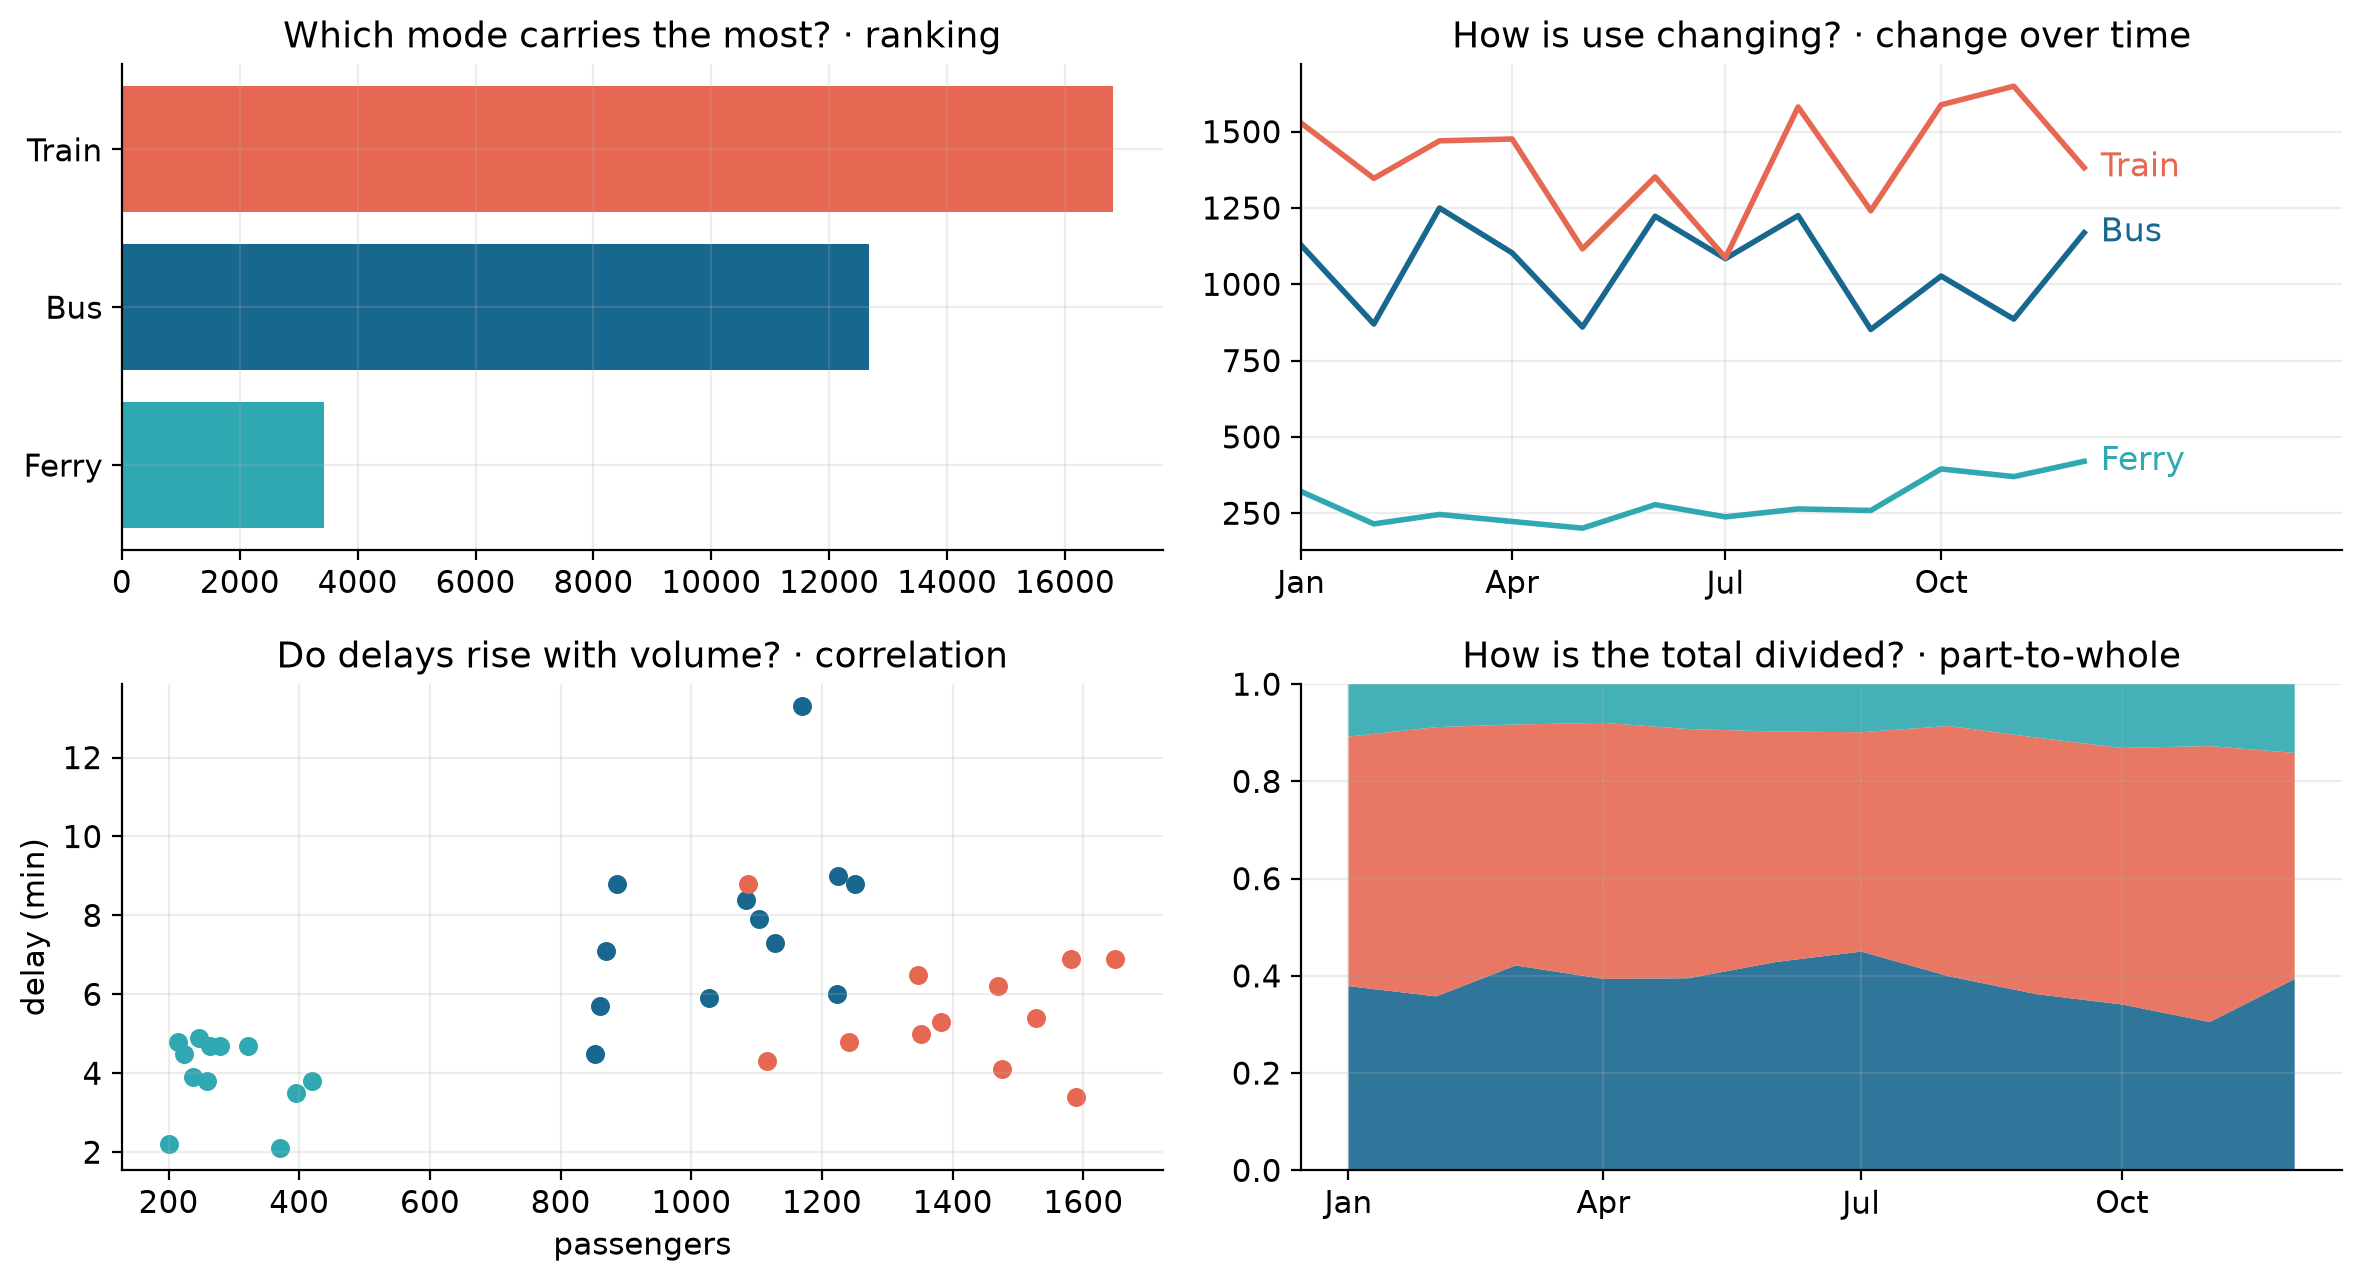
\includegraphics[height=0.56\textheight]{fig-hook.png}\\[0.25em]
  {\small \alert{audience $\rightarrow$ question $\rightarrow$ task $\rightarrow$ data shape $\rightarrow$ form} — not data $\rightarrow$ favourite chart}\\[0.15em]
  \credit{Synthetic transport table: monthly bus, train and ferry passengers and delays, 2025 — the dataset you tidy in the notebook.}
\end{frame}

% ---------- 4 · outcomes ----------
\begin{frame}{Goals}
  \begin{enumerate}
    \item Classify fields by type and role.
    \item Rank visual channels by precision.
    \item Turn questions into tasks and forms.
    \item Choose palettes from data semantics.
    \item Reshape wide data to tidy, and verify.
    \item Complete a Chart Choice Decision Record.
  \end{enumerate}
\end{frame}

% ---------- 5 · data types ----------
\begin{frame}{Data types}
  \footnotesize
  \setlength{\tabcolsep}{4pt}
  \begin{tabular}{@{}p{0.22\textwidth}p{0.42\textwidth}p{0.28\textwidth}@{}}
    \toprule
    \textbf{Type / role} & \textbf{Legitimate reading} & \textbf{Example} \\
    \midrule
    nominal & same or different; no order & transport mode · region \\
    ordinal & higher or lower; spacing unknown & Mohs rank · service tier \\
    quantitative, interval & differences meaningful; zero arbitrary & temperature in °C \\
    quantitative, ratio & differences, ratios, true zero & passengers · dollars \\
    temporal & sequence, interval, duration & month · timestamp \\
    spatial / relational & location, connection, transfer & coordinates · links \\
    \bottomrule
  \end{tabular}
  \vspace{0.8em}

  A type can \alert{rule out} an invalid comparison. It cannot select a chart
  without an audience and a question.
\end{frame}

% ---------- 7 · Bertin ----------
\begin{frame}[t]{Bertin's variables}
  \begin{columns}[T]
    \begin{column}{0.56\textwidth}
      \centering
      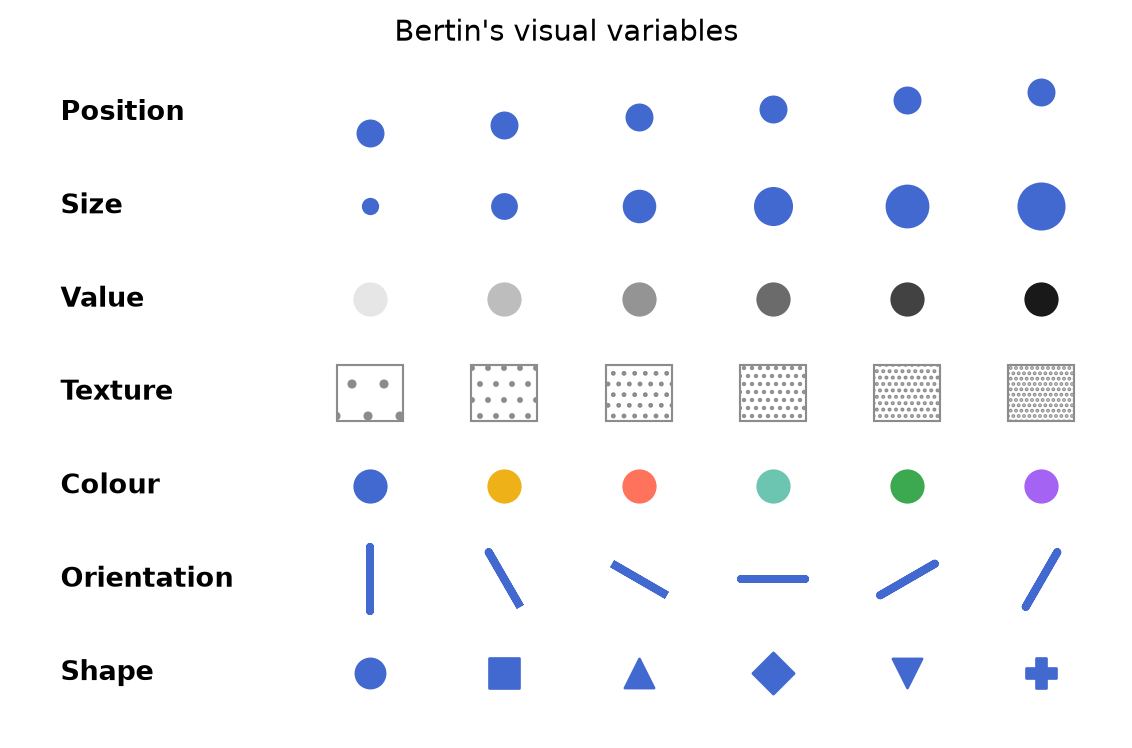
\includegraphics[width=\textwidth,height=0.6\textheight,keepaspectratio]{fig-bertin-output-1.png}
    \end{column}
    \begin{column}{0.4\textwidth}
      \footnotesize Seven ways a mark can vary: position, size, value,
      texture, colour, orientation, shape.\\[0.4em]
      Bertin's question for each variable:
      \begin{itemize}
        \item is it \textbf{selective} — can the eye isolate a group?
        \item is it \textbf{ordered} — does it imply a sequence?
        \item is it \textbf{quantitative} — can it carry an amount?
      \end{itemize}
      \vspace{0.4em}
      \credit{After Bertin, Sémiologie graphique (1967). Course rendering.}
    \end{column}
  \end{columns}
\end{frame}

% ---------- 8 · channel precision ----------
\begin{frame}[t]{Channel precision}
  \centering
  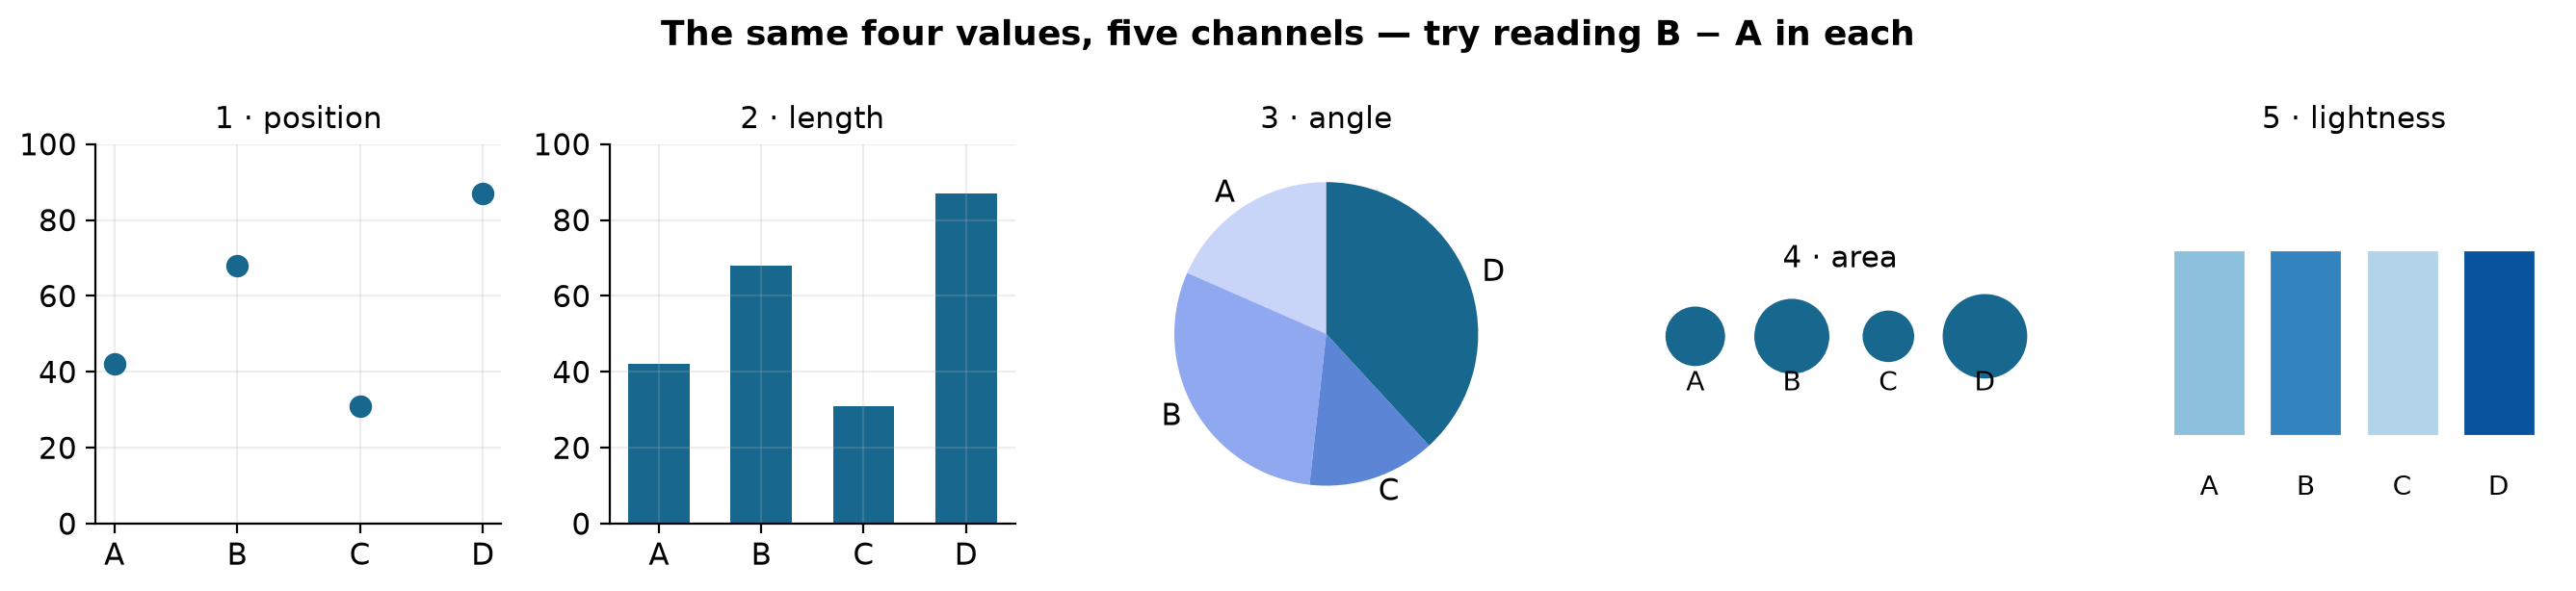
\includegraphics[width=0.98\textwidth]{fig-channels.png}\\[0.4em]
  \begin{flushleft}\small
  Position on a common scale $\rightarrow$ length $\rightarrow$ angle/slope
  $\rightarrow$ area $\rightarrow$ colour lightness.
  The hierarchy is a design aid, not a law detached from audience and task.\\[0.2em]
  \credit{After Cleveland \& McGill (1984).}
  \end{flushleft}
\end{frame}

% ---------- kicker: gallery ----------
\kicker{The Visual Vocabulary}{Nine task families.\\[0.35em]
  {\normalsize The originals on the slides.\\ You rebuild the modern forms in the notebook.}}

% ---------- 10 · deviation ----------
\famframe{Deviation}{rba-budget-balance-2026.png}
  {temporal or categorical + a signed measure with a meaningful zero}
  {variation above and below a fixed reference — zero, a target or an average}
  {diverging bar · surplus/deficit line · spine}
  {Surplus above zero, deficit below. The notebook builds this family from the FRED yield spread.}
  {Reserve Bank of Australia chart pack, Australian Government Budget Balance (\% of GDP) · source: Australian Treasury · © RBA, reproduced with attribution.}

% ---------- 11 · correlation ----------
\famframe{Correlation}{russell-1914.png}
  {two numeric variables, or one numeric + one ordered proxy}
  {direction, form, strength, clusters, outliers}
  {scatterplot · connected scatter · bubble}
  {Note the reversed magnitude axis: bright is up.}
  {H.\ N.\ Russell, Popular Astronomy 22 (1914), Figure 1 · scan courtesy Maria Mitchell Observatory / NASA ADS · public domain.}

% ---------- 12 · ranking ----------
\famframetext{Ranking}
  {categorical identifier + ordinal rank (+ optional true magnitude)}
  {highest, lowest, relative ordered position}
  {sorted bar · sorted dot · bump chart}
  {Mohs published his 1812 scale as a ranked list — no chart existed. Ordinal rank hides that one step near the top is a five-fold jump in true hardness.}

% ---------- 13 · distribution ----------
\famframe{Distribution}{walker-1874-age-sex-deaths.jpg}
  {one numeric variable; optional group (sex) and ordinal bands (age)}
  {range, centre, spread, shape, outliers}
  {histogram · pyramid · box · violin}
  {The 1874 plate shows deaths, not population.}
  {F.\ A.\ Walker, 1874 age-and-sex distribution of deaths · Library of Congress · public domain.}

% ---------- 14 · change over time ----------
\famframe{Change over time}{keeling-curve-noaa-2026-08-05.png}
  {temporal variable + numeric measure; optional category}
  {trend, rate of change, seasonality, turning points}
  {line · slopegraph · area · small multiples}
  {The window is part of the claim: crop it and the story changes.}
  {Scripps Institution of Oceanography + NOAA Global Monitoring Laboratory · 5 Aug 2026.}

% ---------- 15 · magnitude ----------
\famframetext{Magnitude}
  {ordered categories + ratio quantity spanning orders of magnitude}
  {absolute amount on a common (often log) scale}
  {bar · dot · lollipop; area is less precise}
  {After Elton (1927) and Lindeman (1942). It looks like part-to-whole — it is not: \char`~90\% of each level's energy is lost at the transfer, so the tiers sum to nothing.}

% ---------- 16 · part-to-whole ----------
\famframe{Part-to-whole}{fig-topic-mixtures.png}
  {document identifier + topic proportions summing to one}
  {composition within each document and differences between documents}
  {100\% stacked bar · waffle · treemap}
  {Each bar is one document. Its topic shares sum to 100\%.}
  {Document--topic mixtures after Blei, Ng \& Jordan (2003). Course rendering.}

% ---------- 17 · spatial ----------
\famframe{Spatial}{dupin-choropleth-1826.jpg}
  {geometry or location + numeric or categorical attribute}
  {regional pattern, proximity, clustering}
  {choropleth for rates · proportional symbol for counts · dot map}
  {The first modern choropleth. Map rates, not raw counts.}
  {C.\ Dupin, Carte figurative de l'instruction populaire de la France (1826) · BnF · public domain.}

% ---------- 18 · flow ----------
\famframe{Flow}{minard-1869.png}
  {source + target; optional weight and ordered stage}
  {movement, connection, transfer, attrition}
  {Sankey · alluvial · network · route map}
  {Six variables held in one frame.}
  {C.\ J.\ Minard, Carte figurative\ldots (1869) · public domain.}

% ---------- field combinations: the lookup, now the families exist ----------
\begin{frame}{Field combinations}
  \footnotesize
  \begin{tabular}{@{}llll@{}}
    \toprule
    \textbf{Fields} & \textbf{Required comparison} & \textbf{Task family} & \textbf{Common forms} \\
    \midrule
    1 numeric & shape, centre, spread & distribution & histogram · dot · box \\
    1 categorical + 1 numeric & absolute size & magnitude & bar · dot · lollipop \\
    1 categorical + 1 numeric & ordered position & ranking & sorted bar · sorted dot \\
    1 temporal + 1 numeric & trend, rate of change & change over time & line · slope · area \\
    2 numeric & paired association & correlation & scatterplot \\
    1 numeric + 1 reference & signed difference & deviation & diverging bar · residual panel \\
    categories + one total & share of whole & part-to-whole & 100\% bar · ring · treemap \\
    1 spatial + 1 value & regional pattern & spatial & choropleth · prop.\ symbol \\
    source + target (+ weight) & movement, connection & flow & Sankey · alluvial · route map \\
    \bottomrule
  \end{tabular}
\end{frame}

% ---------- 19 · colour dimensions ----------
\begin{frame}[t]{Colour}
  \centering
  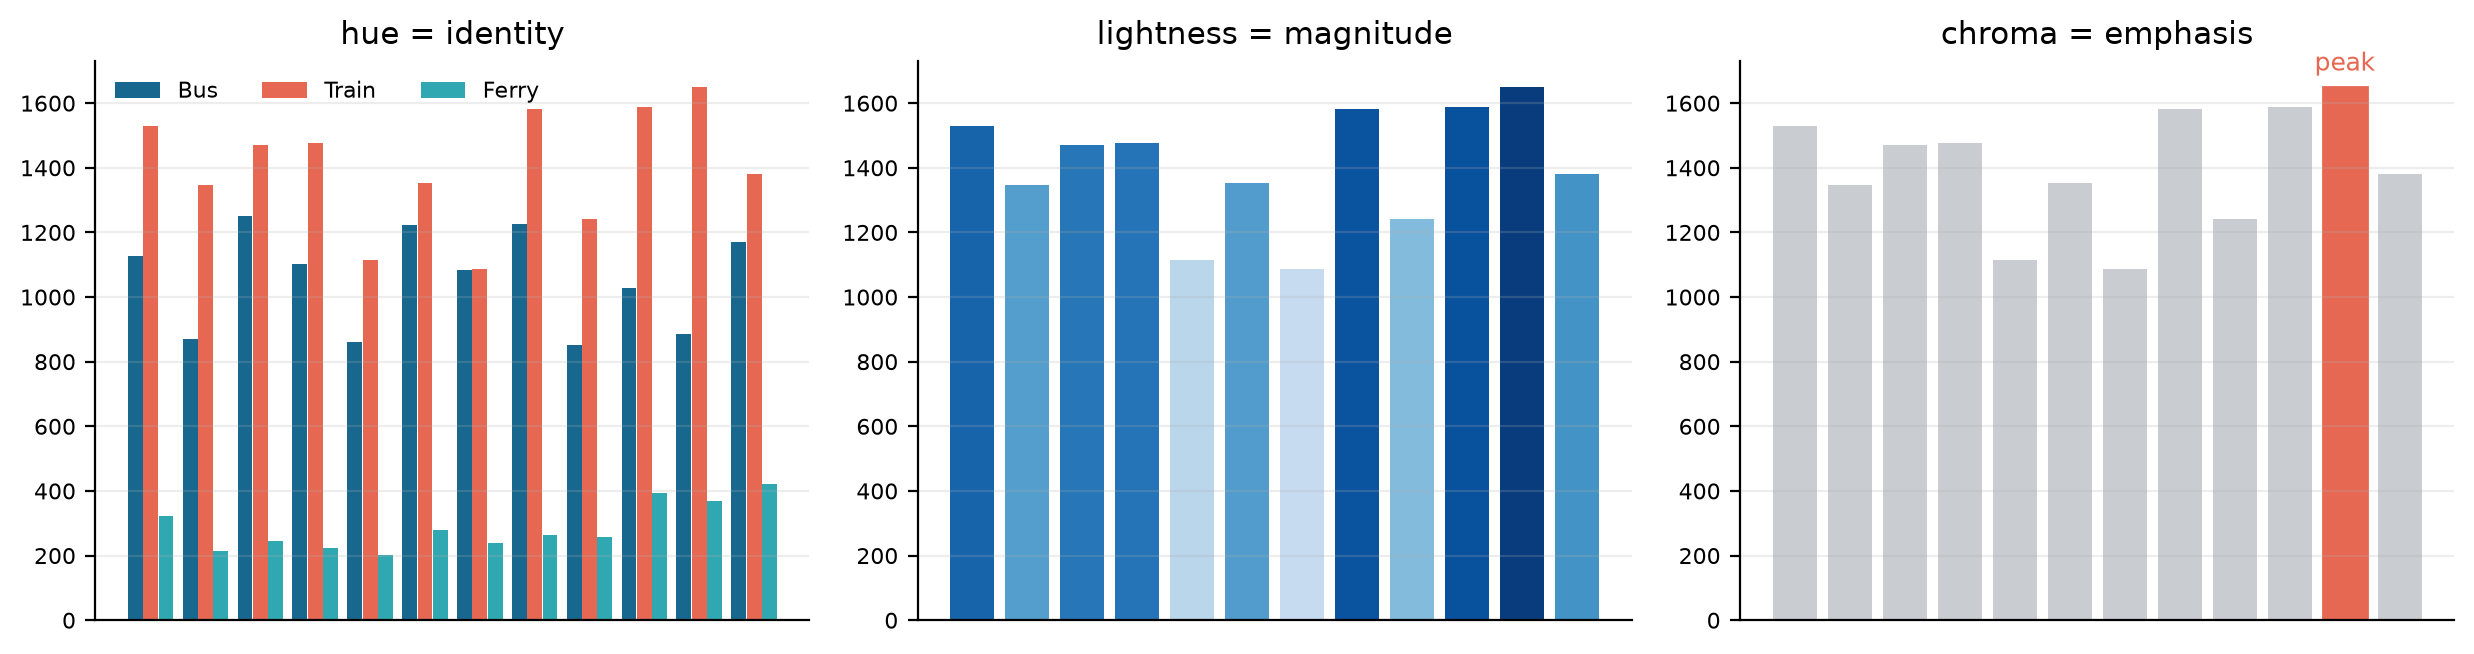
\includegraphics[width=0.97\textwidth]{fig-colour-dimensions.png}\\[0.4em]
  \begin{flushleft}\small
  Colour is contextual and imprecise: let position or length carry exact
  values, and give colour the job it is actually good at.
  \end{flushleft}
\end{frame}

% ---------- 20 · palette families ----------
\begin{frame}[t]{Palettes}
  \centering
  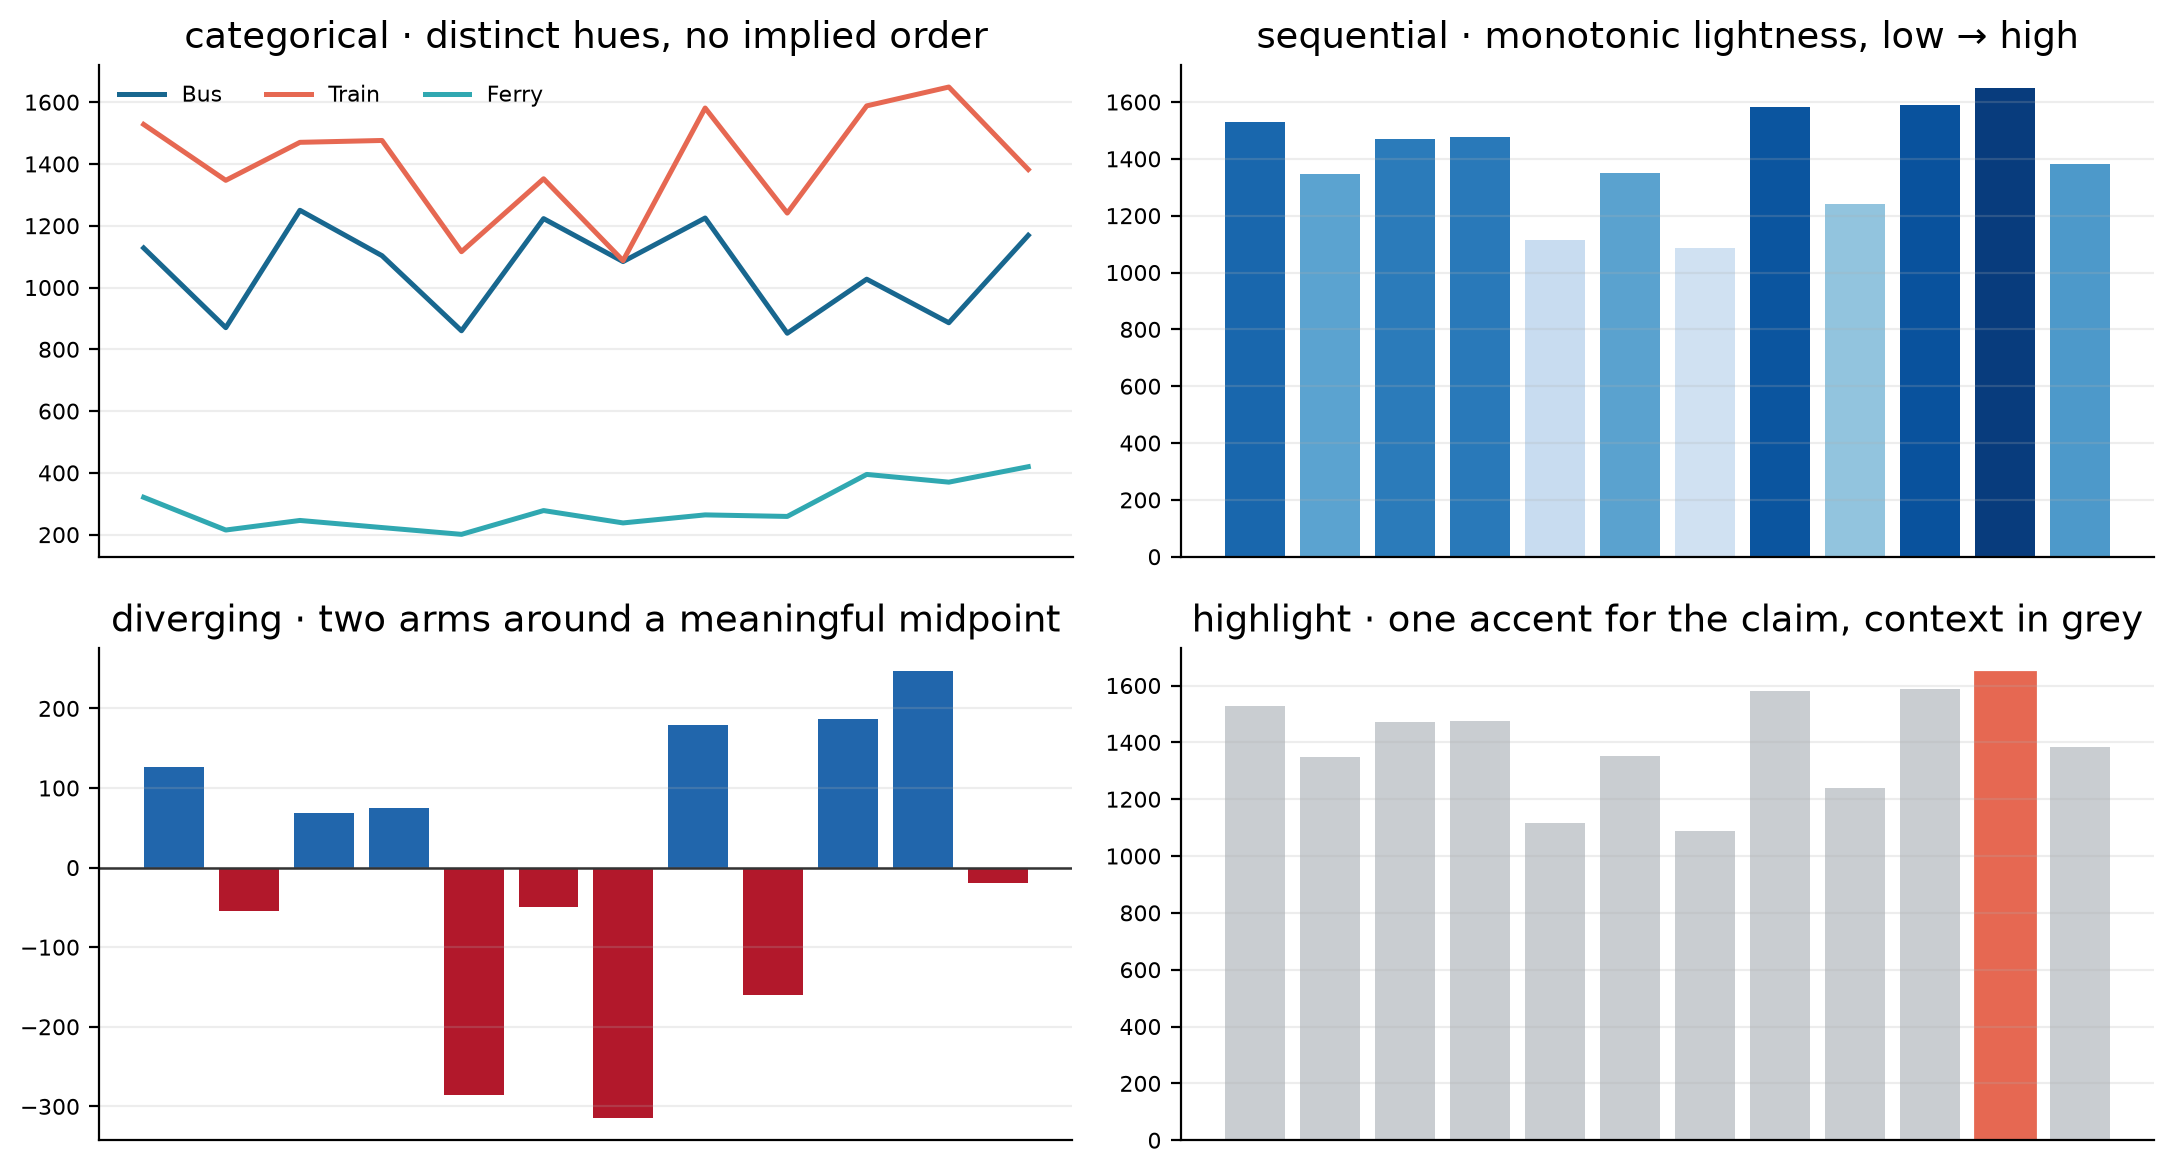
\includegraphics[height=0.53\textheight]{fig-palettes.png}\\[0.25em]
  \begin{flushleft}\small
  The diverging midpoint belongs to the \alert{meaning of the measure} — zero,
  a target, a baseline — never to the palette designer.
  \end{flushleft}
\end{frame}

% ---------- 21 · redundancy ----------
\begin{frame}[t]{Accessibility}
  \centering
  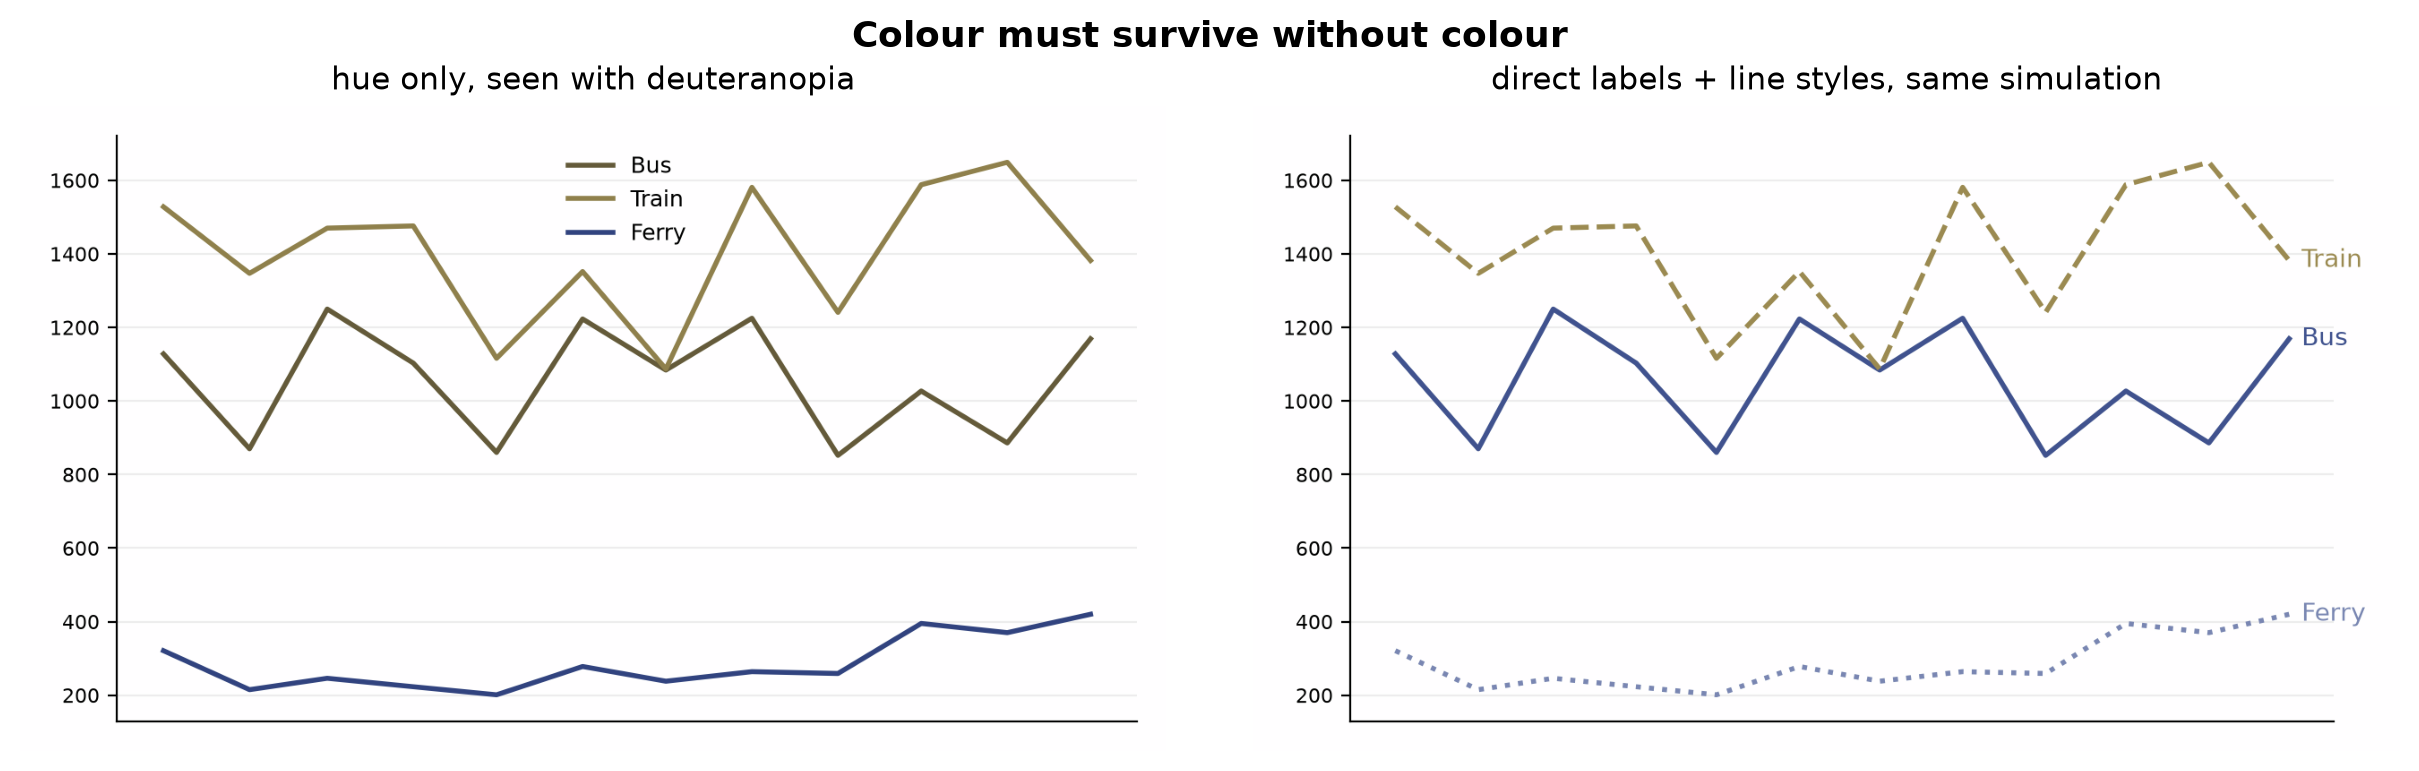
\includegraphics[width=0.93\textwidth]{fig-redundancy.png}\\[0.4em]
  \begin{flushleft}\small
  Add redundant cues: direct labels, line style, shape, position.
  Test the actual chart, not the palette swatch. Distinguish missing from zero.
  Avoid rainbow ramps whose lightness invents boundaries.
  \end{flushleft}
\end{frame}

% ---------- tidy data ----------
\begin{frame}[t]{Tidy data}
  \small Each variable a column · each observation a row · each value a cell.
  \hfill\credit{Wickham (2014)}
  \vspace{0.5em}

  {\footnotesize\ttfamily
  \begin{tabular}{@{}lrrr@{}}
    \toprule
    region & 2023 & 2024 & 2025 \\
    \midrule
    Inner & 1.30M & 1.41M & 1.52M \\
    Western & 1.05M & 1.13M & 1.24M \\
    \bottomrule
  \end{tabular}
  \hspace{1.2em}$\rightarrow$\hspace{1.2em}
  \begin{tabular}{@{}lrr@{}}
    \toprule
    region & year & riders \\
    \midrule
    Inner & 2023 & 1.30M \\
    Inner & 2024 & 1.41M \\
    Western & 2023 & 1.05M \\
    \bottomrule
  \end{tabular}}
  \vspace{0.7em}

  \small The class dataset arrives \alert{deliberately messy}: a `..' sentinel,
  a thousands separator, a missing value. None may be cleaned silently.
\end{frame}

% ---------- 26 · verification ----------
\begin{frame}{Verification}
  \begin{enumerate}
    \item \textbf{Identifiers} — key columns intact; no invented or dropped categories.
    \item \textbf{Row count} — does the reshaped count equal what arithmetic predicts?
    \item \textbf{Types} — numbers numeric, dates dates, no silent strings.
    \item \textbf{Missing} — where did NaNs appear, and are they real or created?
    \item \textbf{Spot totals} — one hand-computed total matches the transformed table.
  \end{enumerate}
  \vspace{0.6em}
  \small The notebook encodes each check as an \texttt{assert} you must satisfy.
\end{frame}

% ---------- 27 · notebook part 1 ----------
\begin{frame}[t]{Notebook Part 1}
  \begin{columns}[T]
    \begin{column}{0.62\textwidth}
      \centering
      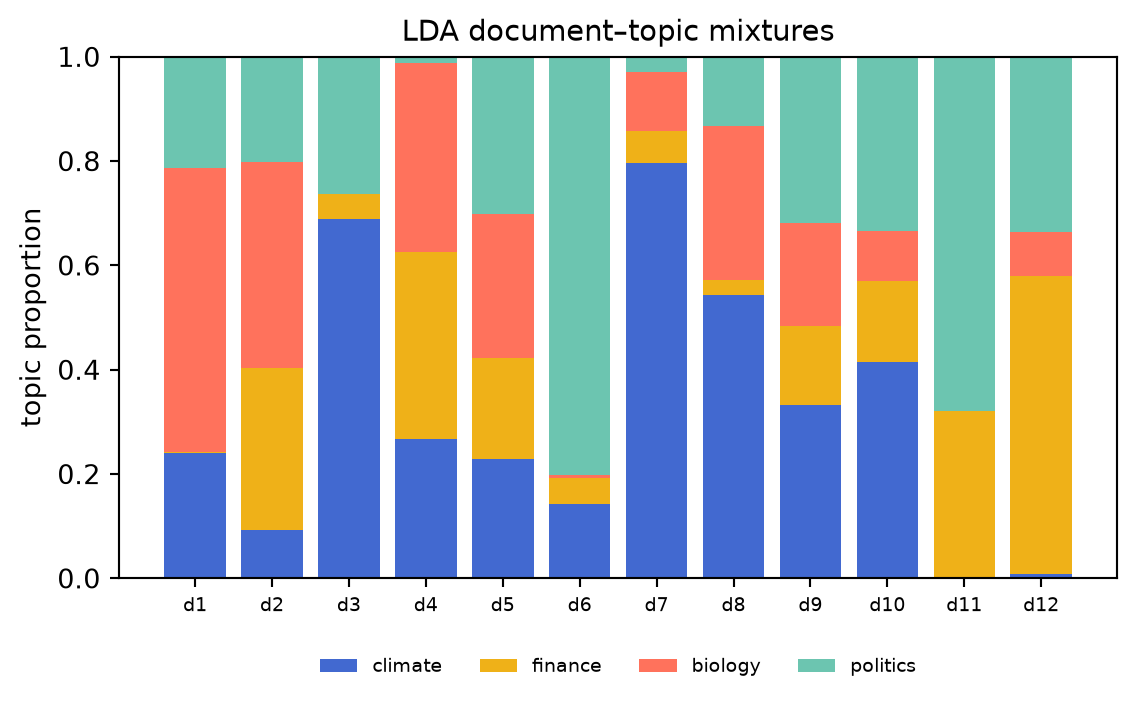
\includegraphics[width=\textwidth,height=0.68\textheight,keepaspectratio]{fig-topic-mixtures.png}
    \end{column}
    \begin{column}{0.35\textwidth}
      {\small \texttt{choosing\_visual\_forms.ipynb}}\\[0.4em]
      \small For each family:
      \begin{enumerate}
        \item run the reconstruction;
        \item satisfy the verification cell;
        \item make one \alert{consequential design intervention} and explain what it changes.
      \end{enumerate}
      \vspace{0.4em}
      \credit{Simulated and representative inputs are labelled; do not cite them as observations.}
    \end{column}
  \end{columns}
\end{frame}

% ---------- 28 · notebook part 2 ----------
\begin{frame}{Notebook Part 2}
  \centering
  {\small \textbf{data types} $\rightarrow$ \textbf{field combinations} $\rightarrow$
   \textbf{required comparison} $\rightarrow$ \textbf{task family} $\rightarrow$ \textbf{form}}
  \vspace{0.7em}
  \begin{itemize}
    \item Name the audience, question and decision \alert{before} naming a chart.
    \item Reshape the messy wide table to tidy long form; pass the five checks.
    \item Build three candidates answering \alert{different questions} — not three styles of one chart.
    \item Select for your claim; reject one plausible alternative for a specific reason.
  \end{itemize}
\end{frame}

% ---------- 29 · A1 bridge ----------
\begin{frame}{A1 Part B}
  \begin{enumerate}
    \item \textbf{Claim} — state a claim the supplied data can support.
    \item \textbf{Task} — name the audience, question and required comparison.
    \item \textbf{Alternative} — design a view that communicates that claim.
    \item \textbf{Compare} — explain what becomes easier and harder to see than in the original.
  \end{enumerate}
  \vspace{0.6em}
  \small The full Chart Choice Decision Record adds the Vocabulary category,
  the supporting field types, and a \alert{genuine rejected alternative} with a
  specific reason. ``It looked worse'' is not sufficient.
\end{frame}

% ---------- exit ----------
\begin{frame}{Exit ticket}
  \begin{itemize}
    \item My audience needs to answer \ldots
    \item This is primarily a \rule{4em}{0.4pt} visual task.
    \item I selected \rule{4em}{0.4pt} because \ldots
    \item I rejected \rule{4em}{0.4pt} because \ldots
  \end{itemize}
  \vspace{0.8em}
  \small Then complete the short open-book diagnostic in Canvas after class.
  It is ungraded and completed without an assistant.
\end{frame}

% ---------- 32 · credits ----------
\begin{frame}[t]{Credits}
  \scriptsize
  \begin{itemize}
    \item Reserve Bank of Australia, chart pack: Australian Government Budget Balance — source Australian Treasury; © RBA, reproduced with attribution.
    \item H.\ N.\ Russell, \emph{Popular Astronomy} 22 (1914), Figure 1 — scan courtesy Maria Mitchell Observatory / NASA ADS; public domain.
    \item F.\ A.\ Walker, age-and-sex distribution of deaths (1874) — Library of Congress, public domain.
    \item Scripps Institution of Oceanography + NOAA GML, Mauna Loa CO\textsubscript{2} record, 5 Aug 2026.
    \item D.\ Blei, A.\ Ng \& M.\ Jordan, latent Dirichlet allocation (2003).
    \item C.\ Dupin (1826) — BnF, public domain. \quad C.\ J.\ Minard (1869) — public domain.
    \item Course renderings: Bertin's variables, HR diagram, Mohs scale, population pyramid, Keeling curve, trophic pyramid, topic mixtures, choropleth and Minard reconstruction.
    \item Reading: FT Visual Vocabulary · Franconeri et al., \emph{The Science of Visual Data Communication} · Wickham, \emph{Tidy Data} · Cleveland \& McGill (1984) · Bertin, \emph{Sémiologie graphique} (1967).
  \end{itemize}
\end{frame}

\end{document}
